%% Figure 4 (pgfplots): Causal baseline-blocking intervention in the full Transformer (clean spacing & outward ticks).
\definecolor{stepc}{HTML}{0072B2}\definecolor{outc}{HTML}{D55E00}\definecolor{theoc}{HTML}{1E7E4E}
\definecolor{modelc}{HTML}{6A3D9A}\definecolor{mutedc}{HTML}{6E6E6E}\definecolor{ctrlc}{HTML}{2B2B2B}
\begin{tikzpicture}[line cap=round, line join=round]
\pgfplotsset{
  every axis/.style={
    scale only axis,
    width=0.240\textwidth,
    height=2.76cm,
    axis line style={black!75, line width=0.64pt},
    tick align=outside,
    tickwidth=2.4pt,
    tick style={black!72, line width=0.52pt},
    tick label style={font=\scriptsize},
    label style={font=\footnotesize},
    ylabel style={yshift=-1pt},
    xlabel style={yshift=1pt},
    title style={font=\footnotesize, at={(0.5,1.04)}, anchor=south},
    axis x line*=bottom,
    axis y line*=left,
    ymajorgrids,
    major grid style={black!7, line width=0.38pt},
    clip=false
  },
  every axis plot/.append style={line width=1.45pt}
}

% (a) Wrong-lag residual correlation E_dist (p = 1/4)
\begin{axis}[
  name=ca,
  title={\textbf{(a)} Distractor noise $E_{\mathrm{dist}}$ ($p{=}\tfrac{1}{4}$)},
  xlabel={Updates ($\times 10^3$)},
  ylabel={$E_{\mathrm{dist}}$ (wrong lags)},
  xmin=0, xmax=1.6, ymin=-0.004, ymax=0.142,
  xtick={0,0.4,0.8,1.2,1.6},
  ytick={0,0.04,0.08,0.125},
  yticklabels={$0$,$0.04$,$0.08$,$0.125$}
]
  \addplot[mutedc, densely dotted, line width=0.75pt, domain=0:1.6, samples=2, forget plot] {0.125};
  \node[anchor=south east, font=\tiny, text=mutedc!95!black, inner sep=1pt] at (axis cs:1.58,0.127) {$\tfrac{1}{2}(1{-}2p)^2$};

  \draw[modelc!65, densely dotted, line width=0.75pt] (axis cs:0.60,-0.004) -- (axis cs:0.60,0.136);
  \node[anchor=west, font=\tiny, text=modelc!92!black, inner sep=1pt] at (axis cs:0.63,0.109) {released ($0.6$k)};

  \addplot[outc, solid] coordinates {
    (0.0,0.1271) (0.1,0.1271) (0.2,0.1271) (0.3,0.1271) (0.4,0.1271)
    (0.5,0.1250) (0.6,0.1073) (0.7,0.0798) (0.8,0.0771) (0.9,0.0626)
    (1.0,0.0443) (1.1,0.0420) (1.2,0.0367) (1.3,0.0355) (1.4,0.0365)
    (1.5,0.0335) (1.6,0.0184)
  };

  \addplot[modelc, densely dashdotted] coordinates {
    (0.0,0.1271) (0.1,0.1271) (0.2,0.1271) (0.3,0.1271) (0.4,0.1271)
    (0.5,0.1250) (0.6,0.1007) (0.7,0.0119) (0.8,0.0103) (0.9,0.0109)
    (1.0,0.0112) (1.1,0.0094) (1.2,0.0070) (1.3,0.0072) (1.4,0.0063)
    (1.5,0.0067) (1.6,0.0048)
  };

  \addplot[stepc, solid] coordinates {
    (0.0,0.1271) (0.1,0.0122) (0.2,0.0122) (0.3,0.0121) (0.4,0.0115)
    (0.5,0.0132) (0.6,0.0162) (0.7,0.0110) (0.8,0.0088) (0.9,0.0042)
    (1.0,0.0038) (1.1,0.0033) (1.2,0.0016) (1.3,0.0014) (1.4,0.0014)
    (1.5,0.0020) (1.6,0.0050)
  };
\end{axis}

% (b) Block-2 true-lag attention share (\delta* = n, p = 1/4)
\begin{axis}[
  name=cb,
  at={(ca.east)}, anchor=west, xshift=1.72cm,
  title={\textbf{(b)} Target-lag share ($p{=}\tfrac{1}{4}$)},
  xlabel={Updates ($\times 10^3$)},
  ylabel={Within-letter lag-$\delta^\star$ share},
  xmin=0, xmax=2.4, ymin=0.08, ymax=0.42,
  xtick={0,0.6,1.2,1.8,2.4},
  ytick={0.125,0.25,0.40},
  yticklabels={$\tfrac{1}{8}$,$0.25$,$0.40$},
  legend style={
    at={(0.5,-0.36)},
    anchor=north,
    legend columns=4,
    font=\scriptsize,
    draw=black!14,
    fill=black!1.2,
    rounded corners=2.8pt,
    inner xsep=6pt,
    inner ysep=2.6pt,
    column sep=6pt,
    cells={anchor=west},
    /tikz/every even column/.append style={column sep=9pt}
  },
  legend image code/.code={
    \draw[#1] (0cm,0cm) -- (0.46cm,0cm);
  }
]
  \addplot[mutedc, densely dotted, line width=0.75pt, domain=0:2.4, samples=2, forget plot] {0.125};
  \node[anchor=south east, font=\tiny, text=mutedc!95!black, inner sep=1pt] at (axis cs:2.38,0.129) {uniform ($1/n$)};

  \addplot[stepc, solid] coordinates {
    (0.0,0.125) (0.1,0.128) (0.2,0.132) (0.3,0.146) (0.4,0.177) (0.5,0.241)
    (0.6,0.287) (0.8,0.324) (1.0,0.338) (1.2,0.353) (1.5,0.360) (1.8,0.375)
    (2.1,0.385) (2.4,0.387)
  };
  \addlegendentry{Standard step ($p{=}\tfrac{1}{4}$)}

  \addplot[outc, solid] coordinates {
    (0.0,0.125) (0.1,0.125) (0.2,0.124) (0.3,0.124) (0.4,0.124) (0.5,0.136)
    (0.6,0.171) (0.8,0.205) (1.0,0.224) (1.2,0.244) (1.5,0.254) (1.8,0.259)
    (2.1,0.260) (2.4,0.266)
  };
  \addlegendentry{Baseline blocked ($p{=}\tfrac{1}{4}$)}

  \addplot[modelc, densely dashdotted] coordinates {
    (0.0,0.125) (0.2,0.124) (0.4,0.124) (0.6,0.171) (0.7,0.210) (0.8,0.217)
    (1.0,0.219) (1.2,0.232) (1.5,0.250) (1.8,0.268) (2.1,0.279) (2.4,0.282)
  };
  \addlegendentry{Released at $0.6$k}

  \addlegendimage{ctrlc, densely dashed, line width=1.18pt}
  \addlegendentry{Symmetric XOR ($p{=}\tfrac{1}{2}$, blocked)}
\end{axis}

% (c) Held-out exact rollout accuracy & p = 1/2 specificity control
\begin{axis}[
  name=cc,
  at={(cb.east)}, anchor=west, xshift=1.66cm,
  title={\textbf{(c)} Rollout accuracy \& $p{=}\tfrac{1}{2}$ control},
  xlabel={Updates ($\times 10^3$)},
  ylabel={Exact rollout (\%)},
  xmin=0, xmax=2.4, ymin=-3, ymax=106,
  xtick={0,0.6,1.2,1.8,2.4},
  ytick={0,25,50,75,100},
  yticklabels={$0$,,$50$,,$100$}
]
  \addplot[ctrlc, densely dashed, line width=1.18pt] coordinates {
    (0.0,0.5) (0.2,0.9) (0.3,12.3) (0.4,29.3) (0.6,38.1) (0.7,55.9)
    (0.8,62.3) (1.1,78.0) (1.5,86.8) (1.6,99.9) (1.8,100.0) (2.1,100.0)
    (2.4,100.0)
  };

  \addplot[stepc, solid] coordinates {
    (0.0,6.5) (0.2,10.5) (0.4,10.6) (0.6,13.9) (0.7,37.5) (0.8,63.5)
    (1.0,74.0) (1.2,89.3) (1.4,91.0) (1.9,93.2) (2.0,99.4) (2.1,100.0)
    (2.4,100.0)
  };

  \addplot[modelc, densely dashdotted] coordinates {
    (0.0,6.5) (0.2,1.7) (0.4,0.6) (0.6,8.7) (0.7,19.1) (0.9,22.1)
    (1.1,39.1) (1.4,53.2) (1.6,68.7) (1.8,73.2) (2.1,72.4) (2.4,73.5)
  };

  \addplot[outc, solid] coordinates {
    (0.0,6.5) (0.2,1.7) (0.4,0.6) (0.6,7.8) (0.7,15.4) (0.8,18.6)
    (1.0,29.3) (1.2,53.7) (1.4,54.3) (1.7,63.6) (2.0,63.9) (2.3,63.7)
    (2.4,70.7)
  };
\end{axis}
\end{tikzpicture}
